%%%%%%%%%%%%%%%%%%%%
\chapter{Signal Processing Theory}
\label{cha:TheThesis}

%%%%%%%%%%%%%%%%%%%%
\section{Modulation from Baseband to RF}

%%%%%%%%%%%%%%%%%%%%
\section{Modulation from RF to Baseband}

%%%%%%%%%%%%%%%%%%%%
\section{Frequency Modulation in Broadcasting}
  %see literature/Present\_lec6\_AM\_FM.pdf\\
  %see lectures out of HSD/ESD

Frequency modulation (FM) is a widely used standard to transmit data streams.
The probably best known usecase therefore is commercial broadcast radio, where an audio stream is transmitted.
Devices to receive these streams are available for low prices to the public.

This chaper describes the main properties of broadcast FM, such as the mathematical description, frequency bands that are used, or the specific frequency parts within a channel spectrum.

%%%%%%%%%%%%%%%%%%%%
\subsection{Mathematical description}

The mathematical description of an FM baseband signal can be described with the formulas presented in this section.
FM encodes the information content in its instantanious frequency.
This means that the measured frequency at any moment in time represents a specific value of a transmitted message.
For a general classification, FM belongs to the group of angle, or phase modulated signals (PM).
The simple reason therefor is, that a frequency has a direct relationship to an angle, if the signal is seen on a unit circle.\\

The instantanious frequency $f_i$ of an FM signal can be described as
\begin{equation}
  f_i = f_c + \Delta f \cdot m(t)
\end{equation}
where $f_c$ is the carrier- or center frequency, $\Delta f$ is the maximum frequency deviation and $m(t)$ is the information or message signal that is to be transmitted.
Simply looking at this equation, the frequency deviation, which is sometimes also called the swing, varies in the range between $f_c \pm \Delta f$.

Considering the relationship between frequency and angle, as described above, and after some simple substitutions which will not be described into detail here, the equation for a generic frequency modulated wave is the following
\begin{equation}
  s(t) = A_c\ cos \Big( 2 \pi f_c t + 2 \pi k_f \int m(t) dt \Big)
  \label{equ:fm_func}
\end{equation}
where $A_c$ is the amplitude of the resulting FM signal and $k_f$ is the frequency sensitivity factor.
This sensitivity factor has a direct relationship with the modulation index $\beta$.
\begin{equation}
  \beta = \frac{\Delta f}{f_m} = \frac{k_f A_m}{f_m}
\end{equation}
where $f_m$ is the highest existing frequency, or the bandwidth of the information signal.
% More info on modulation index: https://fas.org/man/dod-101/navy/docs/es310/FM.htm

Formula \ref{equ:fm_func} describes a frequency modulated signal with a generic message signal $m(t)$.
A widely used example application of FM is broadcast radio, where audio streams are transmitted.
An audio stream can be described as a cosine wave.
Therefor, the information signal that is to be transmitted in broadcast radio can be represented as a cosine wave in the form of
\begin{equation}
  m(t) = A_m\ cos(2 \pi f_m t).
\end{equation}
By inserting this message signal into the generic FM formula \ref{equ:fm_func}, the final equation for an FM signal transforms into the following form.
\begin{equation}
  y(t) = A_c\ cos \Big(2 \pi f_c t + \beta\ sin(2 \pi f_m t)\Big )
\end{equation}
Several formulas, as well as their derivations are described according to \cite{ref_FM_Maths_Info_1}\cite{ref_FMMaths2}.

%%%%%%%%%%%%%%%%%%%%
\subsection{Frequency Band}

The frequency band that is used for FM broadcasting is defined worldwide and spans from 87.5 to 108 MHz.
However, some countries only partially use the band \cite{ref_itu_regulations}.
The range is located within the so-called Very-High-Frequency (VHF) band, which is open to the public in terms of usage.
This means, that any transmitter may use the specified frequency range freely.
Austria allowed the legal usage in 2006 \cite{ref_austria_rundfunkgesetz_2006}.
However, the transmission power needs to be limited, so that neighboring receivers are not disturbed in receiving any existing channels.
The European Commision specifies the power limit as 50 nW of effective radiated power (ERP) \cite{ref_eu_commision_radio_spectrum}.
Another limitation is, that a transmitter must be capable to transmit on multiple center frequencies within the broadcasting band.
It must not be fixed to a single center frequency.
Through this specification, a transmitter is capable of switching its transmission center frequency, in order to avoid interference with another transmitters signal.

In a practical usecase this means that a transmitter needs to select a channel or frequency range, that is not already occupied by an official transmitter.
If a free range is found, the transmitter may start sending an FM signal with the mentioned power limitations \cite{ref_ebu_fm_modulators_in_europe_power_regulations}.

%https://www.ris.bka.gv.at/GeltendeFassung.wxe?Abfrage=Bundesnormen&Gesetzesnummer=20008807


%%%%%%%%%%%%%%%%%%%%
\subsection{Frequency Spectrum of a Broadcast FM Channel}

The entire FM broadcasting band from 87.5 to 108 MHz divides into multiple channels which can be used.
In Europe, the European Telecommunications Standards Institute (ETSI) sets the respective standards for the usage of these frequencies.
The main specifications for a single FM broadcasting channel are explained in this section.\\

Each channel may allocate a bandwidth of 200 kHz.
Within one of these channels, the maximum deviation from the center frequency shall not exceed 75 kHz.
This leaves a guard band of 25 kHz on either side, to minimize interference with adjacent channels.
Center frequencies may be allocated on multiples of 100 kHz.
However, neighboring channels need to be considered therefor, since this may result in an overlap in the spectrum.\\

Fig.\ref{fig_channel_baseband_freqs} shows the frequency spectrum of a single channel, located at its carrier- or center frequency.
For a better overview, only the positive spectum part is shown.
The negative part is an exact mirror, because the transmitted and received signals from the antenna are real signals - they do not have an imaginary part.
The spectrum consists of multiple parts, which are described in the following paragraphs.

\begin{figure}[!h]
  \centering
    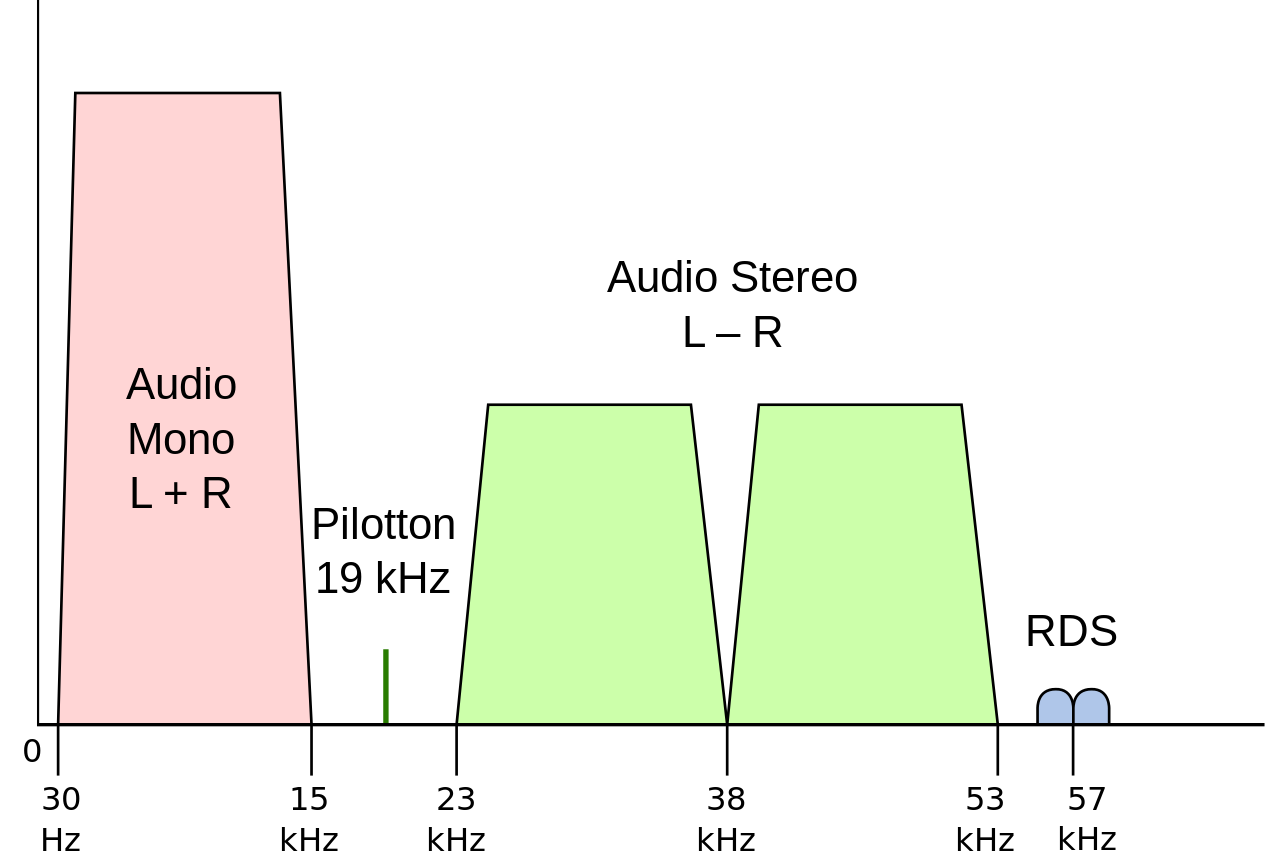
\includegraphics[width=7cm]{img/fm-channel-baseband.png}
  \caption{Allocation of frequencies in an FM channel \cite{ref_fig_channel_freqs}}
  \label{fig_channel_baseband_freqs}
\end{figure}

\subsubsection{Mono Audio Part}

The mono audio stream is located between 30 Hz and 15 kHz.
This signal is built by the sum of the left and right audio channels.
%The lower limit at 30 Hz is to prevent the transmission of a direct current (DC) part, which would require a large amount of power in transmission.
%This effect is one of the downsides of amplitude modulation (AM), where the carrier is located at the channels' center frequeny and requires a high transmission power. % TODO: check this fact
The upper limit at 15 kHz is chosen to maintain a sufficient spacing to the first subcarrier.
For audio streaming, as in FM broadcasting, this is not a limitation, since it is unlikely to have frequencies higher than 15 kHz in an audio stream.
Also, this already reaches the upper limit of the human ears' bandwith, so higher spectral parts will not be heard anyway.

\subsubsection{Pilot Tone}

The first subcarrier is allocated at an offset of 19 kHz from the center frequency.
It is also called the 'pilot tone', since it is a continuous signal.
The pilot tone is used to be able to demodulate the left and right channel of an audio signal correctly, to generate stereo audio.

\subsubsection{Stereo Audio Difference}

A signal that is constructed by the difference between left and right audio channel is modulated on a 38 kHz subcarrier.
This subcarrier is an integer multiple of 19 kHz for practical reasons.
However, the 38 kHz carrier is suppressed and thus not visible in the received spectrum.
It can still be recovered, since it is phase coherent with the 19 kHz pilot tone per definition.
The bandwidth for this difference-signal spans 15 kHz on either side of the subcarrier.
It is used to generate a stereo audio signal, in combination with the mono signal.
This process is explained into more detail in chapter \ref{sec_fm_sig_demod}.

\subsubsection{Additional Services}

Considering all these parts in the spectrum, there is still bandwidth free to use, up to the maximum channel bandwitdh of 100 kHz in one sideband.
Because of that, additional services were added to the pure audio transmission, to provide additional data services and information.
Services that were implemented are the Data Radio Channel (DARC), which is mostly used in Japan and the USA, the Subsidary Communication Authorization (SCA) and the Radio Data System (RDS) \cite{ref_rohde_u_schwarz}.
Out of these, RDS is the most significant service in Europe.
It is used to transmit additional information about the channel, such as the radio stations' name, currently playing songs' title or traffic information.\\

\noindent
The information about the frequency spectrum was taken from \cite{ref_fm_broadcast_tutorial_and_basics}.

%%%%%%%%%%%%%%%%%%%%
\section{Algorithms for Digital FM Demodulation}
  see literature/FmDemodulator.pdf (Sect. 3.3)
  see literature/00476180 Digital FM Demodulator for FM, TV, and Wireless.pdf (Sect. II and III)

  %%%%%%%%%%%%%%%%%%%%
  \subsection{Baseband Delay Demodulator}
  %%%%%%%%%%%%%%%%%%%%
  \subsection{Phase-Adapter Demodulator}
  %%%%%%%%%%%%%%%%%%%%
  \subsection{Phase-Locked Loop (PLL)}
  %%%%%%%%%%%%%%%%%%%%
  \subsection{Mixed Demodulator}
